% Deze template is gemaakt door Fons van der Plas (f.vanderplas@student.ru.nl) voor het publiek domein en mag gebruikt worden **zonder vermelding van zijn naam**.
% This template was created by Fons van der Plas (f.vanderplas@student.ru.nl) for the public domain, and may be used **without attribution**.
\documentclass{report}
\usepackage[utf8]{inputenc}     % for éô
\usepackage[english]{babel}     % for proper word breaking at line ends
\usepackage[a4paper, left=1.5in, right=1.5in, top=1.5in, bottom=1.5in]{geometry}
                                % for page size and margin settings
\usepackage{graphicx}           % for ?
\usepackage{amsmath,amssymb}    % for better equations
\usepackage{amsthm}             % for better theorem styles
\usepackage{mathtools}          % for greek math symbol formatting
\usepackage{enumitem}           % for control of 'enumerate' numbering
\usepackage{listings}           % for control of 'itemize' spacing
\usepackage{todonotes}          % for clear TODO notes
\usepackage{hyperref}           % page numbers and '\ref's become clickable
\usepackage{todonotes}
\usepackage{float}


%%%%%%%%%%%%%%%%%%%%%%%%%%%%%%%%
%% SET TITLE PAGE VALUES HERE %%
%%%%%%%%%%%%%%%%%%%%%%%%%%%%%%%%
%             ||               %
%             ||               %
%             \/               %

\def\thesistitle{Thesis Title}
\def\thesissubtitle{Thesis Subtitle}
\def\thesisauthorfirst{Gizem}
\def\thesisauthorsecond{Aydin}
\def\thesissupervisorfirst{Faegheh}
\def\thesissupervisorsecond{Hasibi}
\def\extthesissupervisorfirst{S. Amin}
\def\extthesissupervisorsecond{Tabatabaei}
\def\thesissecondreaderfirst{name}
\def\thesissecondreadersecond{Surname}
\def\thesisdate{date}


%             /\               %
%             ||               %
%             ||               %
%%%%%%%%%%%%%%%%%%%%%%%%%%%%%%%%
%% SET TITLE PAGE VALUES HERE %%
%%%%%%%%%%%%%%%%%%%%%%%%%%%%%%%%


%% FOR PDF METADATA
\title{\thesistitle}
\author{\thesisauthorfirst\space\thesisauthorsecond}
\date{\thesisdate}

%% TODO PACKAGE
\newcommand{\towrite}[1]{\todo[inline,color=yellow!10]{TO WRITE: #1}}

%% THEOREM STYLES
\newtheorem{theorem}{Theorem}[section]
\newtheorem{corollary}{Corollary}[theorem]
\newtheorem{lemma}[theorem]{Lemma}
\newtheorem{proposition}[theorem]{Proposition}

\theoremstyle{definition}
\newtheorem{definition}[theorem]{Definition}

\theoremstyle{remark}
\newtheorem*{remark}{Remark}


%% MATH OPERATORS
\DeclareMathOperator{\supersine}{supersin}
\DeclareMathOperator{\supercosine}{supercos}

%%%%%%%%%%%%%%%%%%%%%%%

\begin{document}
\begin{titlepage}
	\thispagestyle{empty}
	\newcommand{\HRule}{\rule{\linewidth}{0.5mm}}
	\center
	\textsc{\Large Radboud University Nijmegen}\\[.7cm]
	
\includegraphics[width=25mm]{img/in_dei_nomine_feliciter.eps}\\[.5cm]
	\textsc{Faculty of Science}\\[0.5cm]
	
	\HRule \\[0.4cm]
	{ \huge \bfseries \thesistitle}\\[0.1cm]
	\textsc{\thesissubtitle}\\
	\HRule \\[.5cm]
	\textsc{\large Thesis MSc Computing Science}\\[.5cm]
	
	\begin{minipage}{0.4\textwidth}
	\begin{flushleft} \large
	\emph{Author:}\\
	\thesisauthorfirst\space \textsc{\thesisauthorsecond}
	\end{flushleft}
	\end{minipage}
	~
	\begin{minipage}{0.4\textwidth}
	\begin{flushright} \large
	\emph{Supervisor:} \\
	\thesissupervisorfirst\space \textsc{\thesissupervisorsecond} \\[1em]
	\emph{External Supervisor:} \\
	\extthesissupervisorfirst\space \textsc{\extthesissupervisorsecond} \\[1em]
	\emph{Second reader:} \\
	\thesissecondreaderfirst\space \textsc{\thesissecondreadersecond}
	\end{flushright}
	\end{minipage}\\[4cm]
	\vfill
	{\large \thesisdate}\\
	\clearpage
\end{titlepage}

\tableofcontents



\newpage
\begin{abstract}
    This is the abstract
\end{abstract}
\newpage
\chapter{Introduction}
\label{sec:intro}
Automatic extraction of funding information from academic articles has been an interesting subject for researchers, and various approaches have been proposed for this purpose \cite{ElsPaper,AckExtract,GrantExtractor}. Annotating articles with their corresponding funding information adds significant value to the research community, such as enabling organizations to track the outcome of the research they funded \cite{ElsPaper} and aiding the compliance of open access rules \cite{GrantExtractor}. However, this task is far from trivial, and there is still room for improvement.

Funding information extraction contains subtasks in itself. These can roughly be summarized as:
\renewcommand{\labelenumi}{(\roman{enumi})}
\begin{enumerate}
     \vspace{-0.3cm}\item isolating the piece of text that contains the funding information from the articles,
     \vspace{-0.6cm}\item extracting mentions of funding organizations and grant numbers from the selected text,
     \vspace{-0.3cm}\item linking the funding organization mentions to the corresponding entities in a specific Knowledge Repository to determine which funder is being acknowledged,
     \vspace{-0.3cm}\item linking grant numbers to the respective funder mention to decide which grant number belongs to which funder. 
\end{enumerate}

\vspace{-0.3cm}\noindent In this thesis, the aim is to develop a neural Entity Linker for funding domain, hence tackling subtasks (ii) and (iii).


Entity Linking (EL) is the task of annotating text with corresponding entity identifiers from a Knowledge Repository (KR) \cite{balog}. EL entails Named Entity Recognition (NER) and Named Entity Disambiguation (ED), where the former corresponds to detecting mentions and their respective types from the text and the latter corresponds to linking the mentions to a KR \cite{balog}. 

A large amount of literature addresses EL, NER and ED using neural approaches, which includes the state-of-the-art methods \cite{REL,LUKE,mulang} as well. However, the bigger part of this work focuses on performing these tasks in general-domain, often times considering Wikipedia pages as entities \cite{nlpnotes}. Hence, there is no guarantee that these approaches will perform well in funding domain.

There are significant amount of differences between performing EL in general-domain and in funding domain. First of all, a different knowledge repository is needed as most of the smaller funders do not exist in general-purpose knowledge repositories.  Another challenge is the fact that some information that is deemed highly important in general-domain ED may not be as informative in this domain. For example, \cite{raiman} reported that ED would almost be solved if entity type information could be estimated better. However, in funding domain, some of the most ambiguous mentions are the ones referring to ministries, as a lot of countries may have a ministry with the same name. In these cases, the type of the mentions being, for example, governmental organizations would not provide any clue. 

Funding domain introduces additional challenges for the NER task as well. For example, the mentions of organizations that are not funders should not be extracted. Another challenge is the limited amount of labelled data. In general-domain setting, Wikipedia could be exploited to extract millions of samples \cite{bunescu-pasca-2006-using}. Supervised neural architectures for NER require a large amount of training data to obtain high performance \cite{NERsurvey}.

Considering the mentioned differences, this thesis aims to answer the following research question:

\begin{quote}\emph{RQ: Is it possible to use neural approaches for Entity Linking in funding domain, where labelled data is limited and a domain-specific knowledge repository is used?}\end{quote}

\textcolor{red}{Explain how the research question will be answered and that the data/resources from Elsevier will be used.}

\textcolor{red}{Explain what each section entails.}
\textcolor{red}{Add stuff from Radboud Writing Lab session}
\textcolor{red}{Put some part of this in a section called Research something}
\newpage
\section{Task Definition}
In this thesis, the aim is to perform Entity Linking (EL) in funding domain. Typically, EL consists of two subtasks, Named Entity Recognition (NER) and Entity Disambiguation (ED).

Given a piece of text $d=\{x_1,...,x_N\}$ of $N$ tokens, the task of NER is to identify a set of spans $M = \{m_i \mid m_i = \{x_s,..,x_e\}, s \geq 1 \land s\geq e \land N \geq e\}$, where each span corresponds to an object, person or even a piece of information of interest. These spans are called named entities, or mentions. Usually, detecting the types of the extracted mentions is also part of the NER task. The available mention types differ among systems based on their objectives. In this thesis, each mention $m_i$ corresponds to either a \textit{Funding Organization} ($ORG$)  or a \textit{Grant Number} ($GRT$). Hence, $type(m_i) \in \{ORG,GRT\}$. Throughout this research, it is assumed that the mentions are not nested and are not overlapping.

Given the set of mentions $M$, the aim of ED is to link each mention to their corresponding entity $e_i \in \mathcal{E} $ in a knowledge repository. A knowledge repository is a collection of entities, and may contain information on the entities and relations between them. The contents and specifications of the knowledge repository used is task-dependent. The task of ED is not trivial as many different mentions may be used to refer to the same entity, or the same mention may be used to refer to different entities. When the correct link of a mention $m_i$ is entity $e_i$, this will be denoted as $link(m_i) = e_i $.  Another thing to note is that some mentions may not correspond to any entity in the target knowledge repository. These mentions are usually referred to as \textit{NIL Mentions}. To denote these cases, a NIL entity $\emptyset \in \mathcal{E}$ will be used. In this thesis, a knowledge repository of funding organizations is used, hence, only the mentions with type $ORG$ will be considered for ED.

Sometimes, the set of entities $\mathcal{E}$ may be extremely large. In that case, a Candidate Selector (CS) may be used to limit the search space. The aim of the CS is to extract a set of candidate entities $C_i = \{e_1,...e_K\} \subset \mathcal{E} $ for a given mention $m_i$. Usually the size of $C_i$ is much smaller than that of $\mathcal{E}$. This enables using more complex algorithms for ED as it reduces the number of entities to consider.

Lastly the task of EL, which is the aim of this thesis, is to extract a set of mention-entity pairs from an input text $d$. In this thesis, as only the $ORG$ mentions will be linked, the objective can be defined as exracting the set $T = E_{ORG} \cup M_{GRT}$ for each input $d$, where,
\begin{equation}
E_{ORG}=\{(m_i,e_i) \mid m_i \in M \land e_i \in \mathcal{E} \land link(m_i)=e_i \land type(m_i) = ORG\}
\end{equation}
and 
\begin{equation}
M_{GRT} = \{m_i \mid m_i \in M \land type(m_i) = GRT\}.
\end{equation}
\newpage
\chapter{Related Work}
There is a large amount of literature on Entity Linking and its subtasks, Named Entity Recognition and Named Entity Disambiguation. The bigger part of this literature focuses on performing these tasks in the general-domain setting, often times considering Wikipedia pages as entities \cite{nlpnotes}. While this line of research introduces the state-of-the-art approaches, there is no guarantee that these approaches will perform well in a domain-specific setting with a custom knowledge repository. Hence, domain-specific literature is also investigated to get insights on adapting general-purpose methods to specific domains.

Section \ref{FundingDataExtraction} reviews the literature on automatic funding information extraction from academic articles. In Section \ref{sota}, state-of-the-art general-purpose NER, ED and EL solutions are presented. Domain-specific neural NER, ED and EL approaches are demonstrated in Section \ref{domSpec}. Section \ref{entityRep} concentrates on entity representations in neural ED, mainly entity embeddings, and lastly, Section \ref{preLMDiffDomain} reviews the literature on using pretrained neural language models in domain-specific applications.
\section{Funding Information Extraction}
\label{FundingDataExtraction}

    One of the most notable work on automatically extracting funding information from text is FundingFinder \cite{ElsPaper}. FundingFinder is a two-step pipeline that utilizes NLP techniques. In the first step, the paragraphs that contain funding information are determined, and in the second step, NER is performed using an ensemble of different Sequential Learning approaches. The authors also created a publicly available benchmark dataset for this task. The approach used in this thesis builds upon this work, keeping the first step intact while improving the second step, and adding the ED capability. 
    
    Before FundingFinder, not much literature existed on extracting funding information from text automatically, and the existing work mostly utilized regular expressions \cite{ElsPaper}. Recently, there have been more approaches presented to tackle this problem. In 2020, Wu et al. proposed AckExtract  \cite{AckExtract}, which extracts funder organization mentions from the COVID-19 Open Research Dataset \cite{CORD}. For NER, they use a pretrained neural model from the package Stanza \cite{stanza}, which uses Contextual String Embeddings \cite{flairpaper}. However, their method does not include any ED, whereas in this thesis, one of the tasks is to link the funder mentions to their corresponding entities in the domain-specific Knowledge Repository. Another approach is proposed in 2021, GrantExtractor \cite{GrantExtractor}, which extracts funding information from articles in biomedical literature, in the form of grant numbers and their corresponding organizations. For extracting grant numbers, they train a BiLSTM-CRF \cite{BiLSTMCRF} architecture. Using a multi-class classifier, they determine which organization the extracted grant number belongs to. They do not use any neural approaches for extracting organization mentions. Also, the focus of GrantExtractor is on linking grant numbers to their respective organizations, while the focus of this thesis includes extracting all funding organizations that financially supported the corresponding research, even though no grant information is acknowledged.

\section{Entity Linking and Subtasks}
\label{sota}
In this section, the current state-of-the-art methods for EL and its subtasks are investigated \footnote{\url{http://nlpprogress.com/english/entity_linking.html}}.
\subsubsection{Named Entity Recognition}
In the past couple of years, Deep Learning has been a popular choice to tackle the NER problem, and the corresponding research has improved the state-of-the-art results \cite{NERsurvey}. In 2018, Akbik et al. proposed Contextual String Embeddings \cite{flairpaper}, which represents words using a character-level neural language model, and is able to produce different word embeddings depending on the context. By utilizing a BiLSTM-CRF architecture that takes the concatenation of Contextual String Embeddings and pretrained GloVe embeddings \cite{glove} as input, they report state-of-the-art results in both German and English NER, in the CoNLL-2003 \cite{conll} setup. In 2019, Devlin et al. introduced BERT \cite{BERT} which obtained new state-of-the-art results on several tasks. In English CoNLL-2003, they obtained an F1 score of $92.8\%$ using the cased version of BERT$_{BASE}$\cite{BERT}, performing very close to \cite{flairpaper}, which obtained $93.1\%$.

Some approaches for NER utilize external resources, such as a list of entity names, which may be called a dictionary or a gazetteer. This may boost the performance of the system, but may also hurt the generalization ability \cite{NERsurvey}. However, there have been various models presented \cite{NERgazetteer, NERDict} that incorporate this information while performing comparable to \cite{flairpaper}. With this approach, both papers \cite{NERgazetteer, NERDict} aim to improve the performance on entities that do not appear in the training set or that are rare. 

Recently, Yamada et al. (2020) proposed LUKE \cite{LUKE}, a contextualized representation for both words and entities, to be used in entity-related tasks. LUKE is based on the bidirectional transformer \cite{transformer}, however, it treats words and entities as independent tokens. For this purpose, the authors propose a modified attention mechanism as well as a new training methodology based on BERT's \cite{BERT} masked training. They pretrain LUKE using a large entity-annotated Wikipedia corpus. By using the proposed embeddings, they report the new state-of-the-art results for NER, improving upon \cite{flairpaper}.

\subsubsection{Named Entity Disambiguation}

In 2018, Raiman and Raiman proposed DeepType \cite{raiman}, an ED approach, a neural network that is constrained by the predicted type information for a given entity. By using the type information, they also reduce the complexity of disambiguation from polynomial to linear. DeepType produced state-of-the-art results in three ED datasets, by obtaining scores of 92.36\%, 94.88\% and 90.85\% on WikiDisamb30 \cite{wikidisamb}, CoNLL (YAGO) \cite{CoNLLYago} and TAC-KBP-2010\footnote{\url{https://tac.nist.gov/}} respectively. The authors also note that DeepType can reach 99.0\% and 98.6\% accuracy on CoNLL (YAGO) and TAC-KBP-2010, when the type information is provided by an Oracle. Based on that, they claim the ED problem can almost be solved if the type classifier is improved. However, in the case of funding domain, most of the ambiguities in mentions cannot be solved by using the type information. For example, the mention ``Ministry of Health'', can be resolved to different entities corresponding to ministries in different countries, however,  the types of these entities would be the same.

The paper proposed by Mulang' et al. (2020) \cite{mulang} slightly advances the state-of-the-art ED results for CoNLL (YAGO) \cite{CoNLLYago} dataset by obtaining a score of 94.94\%. The authors introduce the idea of incorporating context derived from Knowledge Graphs (KG) to pretrained transformers with the aim of improving their performance for ED. They extract triplets from the KG, verbalize them into natural language form, and append them to the input sentence and mention before passing it through the transformer. When they replace the Wikipedia description used in the DCA-SL model \cite{dca} with the structured KG context they extracted, they obtain the above-mentioned score. 

Another interesting approach is proposed by Wu et al. in 2020 \cite{scalablezeroshot}, which outperforms DeepType \cite{raiman} in TAC-KBP-2010 by obtaining a 94.5\% accuracy . Their method also achieves state-of-the-art results in the zero-shot Entity Linking dataset derived from WikilinksNED \cite{wikilinksned}. To perform ED, they only use textual information and architectures that utilize pretrained BERT \cite{BERT} transformers. They represent the mention using itself and its context, and the entity using its description. Using a bi-encoder \cite{polyencoders}, they encode the mention and entity representations in the same space, which they later use to extract candidates for a given mention using approximate nearest neighbor search. They make the final decision by passing representations of the candidate entities and mentions through a cross-encoder \cite{polyencoders}. 

\subsubsection{Entity Linking}
Kolitsas et al. (2018) \cite{kolitsas} proposed the first end-to-end neural EL system in 2018, and recorded state-of-the-art results in AIDA CoNLL dataset \cite{CoNLLYago}. By tackling NER and ED jointly, the authors aim to utilize the dependency between these two tasks. They suggest that this has several benefits, such as improved mention boundary recognition. Their method first extracts all possible mention spans from the input. Then, the model computes a score for each mention - candidate entity pair, using pretrained entity embeddings \cite{kolitsasEmbed}, context-aware mention representations, commonness and long range attention scores. The final output for the input text is based on these scores and global entity coherence. 

In 2020, van Hulst et al. proposed REL \cite{REL}, an EL toolkit that utilizes state-of-the-art NLP research, outperforming \cite{kolitsas} in terms of micro-F1 score in AIDA CoNLL dataset \cite{CoNLLYago}. REL tackles the EL problem in three steps: NER, candidate selection and ED. For NER, they utilize Flair, namely, the sequence labelling architecture and Contextual String Embeddings proposed by \cite{flairpaper}. For each mention, up to 4 candidates are selected using commonness, and up to 3 candidates are selected based on the similarity between the context of the mention and entity embeddings. Entity embeddings are provided by \cite{kolitsasEmbed}, the same ones used in \cite{kolitsas}. For ED, Ment-norm by Le and Titov \cite{mentnorm} is used. Apart from obtaining state-of-the-art results, REL also offers a modular architecture, allowing easy replacement of components and it does not require a GPU during inference time \cite{REL}. 

Broscheit (2020) \cite{bertEL} proposed an architecture that jointly does NER and ED using BERT \cite{BERT}. In this approach, the task of EL is framed as a per-token multi-class classification problem. The model utilizes a pretrained BERT model and an output classification layer on top of it. Even though this approach is a big simplification on the EL task, it performs only a few percents off compared to \cite{kolitsas}.  However, as each entity is cast as a class, the model cannot disambiguate unseen entities. In real-word, knowledge repositories keep growing, and hence it is important for the system to be extendable for entities that do not exist in the training set \cite{gupta}. Moreover, some training datasets may not cover the whole entity vocabulary, such as the one used in this thesis.

\section{Domain-Specific Systems}
\label{domSpec}
In this section, the research that aims to tackle EL, NER and ED in a domain-specific setting with neural architectures will be reviewed.

For NER, there is a great amount of research in general domain, however, more research on domain-specific solutions is expected for supporting real-world applications \cite{quote1}. Existing NER approaches rely on a large amount of annotated data, which may not be available for the domain-specific setting \cite{NERDict2}. Hence, Shang et al. (2018) \cite{NERDict2} proposed AutoNER, a neural architecture that is designed to learn from data that is created by distant supervision, without any human effort. AutoNER uses domain-specific dictionaries to automatically generate labelled data with distant supervision. The authors also introduce the ``Tie or Break'' tagging schema, that is based on predicting whether two adjacent tokens belong to the same mention or not. They reason that this tagging scheme is suitable to use noisy labels generated by distant supervision. They show the effectiveness of their work in multiple datasets, two of them being the BC5CDR \cite{bc5cdr} and NCBI-Disease \cite{ncbi} datasets from the biomedical domain, in which AutoNER achieves 84.8\% and 75.52\% F1-score respectively.

Another domain-specific NER approach that utilizes a dictionary is proposed by Wang et al. (2019) \cite{MedDict}, which tackles the Clinical NER problem in Chinese text. They show the effect of incorporating dictionary knowledge in the BiLSTM-CRF \cite{BiLSTMCRF} architecture on rare and unseen entities experimentally. Also, they suggest five different methods of using dictionaries in this context and compare the results. 

There also exist research on tackling the domain-specific ED problem with neural architectures. In 2019, Mondal et al. \cite{MedicalTriplet} proposed a system that is based on string similarity to perform ED on disease names. The authors utilize a two-step solution. First, for each mention, they extract a set of candidate entities based on Jaccard overlap and the cosine similarity between the entity label and the mention. They use word embeddings to calculate the cosine similarity. For multi-word strings, they sum the embeddings for each word. Then, they rank the candidate entities with a Triplet Network \cite{tripletNetwork}, that learns to reduce the distance of the mention with the positive candidate, while increasing the distance with the negative candidate. As an input to this network, word embeddings is used again to represent the mention and the candidate entity's label. With this approach, they obtain 90\% accuracy on the NCBI-Disease \cite{ncbi} dataset, outperforming previous approaches. 

The input representation of entities vary between different approaches. In another research tackling clinical ED by Schumacher et al. (2020) \cite{ClinicalConcept}, different from \cite{MedicalTriplet},  multi-word strings are represented by two different methodologies, maxpooling over the word embeddings and running self-attention. The authors report that running self-attention produces better results compared to maxpooling. Instead of combining different vectors, Sung et al. (2020) \cite{sung-etal} represents each mention and each synonym of an entity using two different vectors, one that is based on TF-IDF scores, and another that is based on BERT \cite{BERT}. For the latter, the [CLS] token is used to represent the whole phrase. Instead of combining these two vectors, they define two different similarity function for each. The final similarity of a mention and an entity synonym is defined based on the weighted average of these two similarity scores.

Architectures utilizing the type information are also present. Zhu et al. (2020) introduced LATTE \cite{latte}, an architecture for ED in medical domain. The authors emphasize the importance of fine-grained types in their setting, and as this information is not available, they model the fine-grained types as latent variables. For ED, in addition to the latent fine-grained types, they use the similarity between the entity's label, and the mention and its context. To train their model, they use multi-task learning for both type classification and ED.

Some proposed methodologies tackle the EL problem as a whole in a domain-specific setting using neural architectures. For biomedical domain, Zhao et al. (2019) \cite{MedFeedback} proposed a joint neural architecture for NER and ED tasks for performing EL. Their architecture utilizes explicit feedback between the two tasks in a multi-task learning setting. With this architecture, they obtain F1 scores of 87.43\% and 88.23\% in NER and ED tasks of the NCBI-Disease \cite{ncbi} dataset respectively, and 87.62\% and 89.17\% in BC5CDR \cite{bc5cdr} dataset. With these numbers, they outperform AutoNER \cite{NERDict2} in NER setting for both datasets, and perform comparable to \cite{MedicalTriplet} in NCBI-Disease dataset for ED.

Biomedical domain is not the only one in which neural approaches are used for NER, ED and EL. In 2019, Espejo-Garcia et al. \cite{agricultural} proposed a solution to extract named entities that refer to the important parts of phytosanitary regulations, which is related to the agricultural domain. The authors experimented with eight different state-of-the-art neural architectures. For their setting, the best performing architecture was a bidirectional LSTM \cite{bilstm} that utilized a Softmax layer for inference and got the concatenation of pretrained Word2Vec \cite{w2v} embeddings with character based word representations as input. With this architecture, they obtained an F1 Score of 88.3\%. Apart from agricultural domain, Yang et al. (2020) \cite{cosmetic} proposed Headword Oriented Entity Linking, an EL setting where the mention scopes do not need to be identified, to extract cosmetic products from blogs and to disambiguate them to a domain-specific knowledge repository. First, using word segmentation techniques, they identify the headwords of the mentions. Then, they apply classification on the mentions to decide whether the mention can be linked to a product that is in the knowledge repository. Lastly, they use a modified version of the architecture proposed by \cite{gupta} for ED.  Another interesting study is by Kurz et al. (2020) \cite{TechTickets}, where they experiment with different BERT-based \cite{BERT} architectures to disambiguate mentions of machine parts and errors belonging to German technical service tickets.

\section{Entity Representation}
\label{entityRep}
In neural ED, entity representation plays an important role. Some research frames the problem as multi-class classification and represent entities as different classes \cite{bertEL,MedDiffArc,MedFeedback}, while other research tends to use architectures that takes properties of entities as input and learns a representation internally during training for ED \cite{scalablezeroshot}, implicitly or explicitly. Another line of research utilizes entity embeddings \cite{REL,kolitsas,dca,MedicalTriplet}. In this section, the literature on entity embeddings will be reviewed.

There is a large body of literature on embedding entities and relations found in knowledge repositories. One of the most notable work is TransE \cite{TransE}, introduced in 2013. TransE generates embeddings for each entity and relation in the input knowledge repository. The idea behind TransE is to model relations as translations in the embedding space. For a given triplet $(h,l,t)$ in the knowledge repository where $h$, $l$ and $t$ denote head entity, relation and tail entity respectively; TransE aims to make the embedding of $t$ as close as possible to the sum of the embeddings of $h$ and $l$, using an energy-based model. Later on, there has been models that improved upon TransE such as TransH, TransR, CTransR and TransD, each improving upon the previously proposed one respectively  \cite{TransEimproved}. Another interesting work that generates entity embeddings utilizing the triplets in knowledge repositories is RDF2Vec \cite{RDF2Vec}. RDF2Vec extracts graph sub-structures, and treats them as sentences to train a Word2Vec \cite{w2v} model. 
 
In 2017, Gupta et al. \cite{gupta} proposed a neural architecture that can generate entity embeddings that jointly encodes the information on the entity's description, the context of its mentions and its type. The architecture consists of three models that encode the different information. The parameters of the models and the embeddings are jointly learned based on the sum of four different losses that ensure the entity embeddings and the encoded information is similar. The summation guarantees that entity embeddings can be generated even though some information is missing, such as the description \cite{gupta}. They also proposed an ED model based on these embeddings. As mentioned in Section \ref{domSpec}, a modification of this architecture is used to create entity embeddings in \cite{cosmetic}. Another interesting neural approach for generating entity embeddings was proposed by Ganea and Hofmann in 2017 \cite{kolitsasEmbed}, and, their pretrained entity embeddings have been used by research that reported state-of-the-art results in EL \cite{REL, kolitsas}. In their approach, the words and entities are embedded in the same space by extending a pretrained Word2Vec model \cite{w2v} to cover entities as well. They generate the entity embeddings such that they are close to the vectors of the words that occur in the corresponding entity descriptions and in the mention contexts that belong to the entity. 

Gillick et al. (2019) \cite{googleintern} proposed a dual encoder architecture for ED, which also learns entity embeddings. The model has one encoder to encode the mention and its context, another encoder to encode the entity using its description and categories. Then, the model is trained to maximize the cosine similarity between the encoded representations of the correct mention - entity pairs. After training, the entity embeddings are precomputed using the entity encoder and stored for inference. 

Another successful method to get entity embeddings is Wikipedia2Vec \cite{wikipedia2vec2}. They also have pretrained embeddings available for use. Wikipedia2Vec encodes words and entities in the same space and utilizes Word2Vec \cite{w2v}. To train Wikipedia2Vec, they use three models. Word-based skip gram model puts the embeddings of words that occur in similar context close, anchor context model puts the embeddings of entities close to embeddings of words that occur near the anchor texts of the entity, and lastly, link graph model puts the entity embeddings close based on Wikipedia's hyperlink graph. 





\section{Using Pretrained Language Models in Domain-Specific Applications}
\label{preLMDiffDomain}
BERT \cite{BERT}, and other pretrained language models have been used extensively in various NLP applications and have obtained state-of-the-art results in benchmark tasks \cite{pretrainedLM}. However, for some domains, they may be too generic and may not be able to cover specific needs \cite{quote2}. Hence, it may be worthwhile to adapt the pretrained language model that will be used to the specific domain. Gururangan et al. (2020) \cite{DontStop} shows that a second-round of pretraining of a pretrained language model improves the performance in both low and high resource settings, using different domains and tasks. Also, Fraser et al. (2019) \cite{quote3}, reports that language models which are pretrained with domain-specific text perform better on the task of NER in biomedical domain. However, it should be noted that training a neural language model from scratch for a specific domain can take weeks \cite{tritrain}. 

There is emerging research on cheap domain adaptation of pretrained language models. Gururangan et al. (2020) \cite{DontStop} proposed Task-Adaptive Pretraining (TAPT), which corresponds to pretraining the neural language models further with the unlabeled data of the task at hand. They report that this approach performs comparable to pretraining with larger amount of text from the same domain. Tai et al. (2020) proposed exBERT \cite{exBERT}, a low-cost method to add new domain-related words to the vocabulary of BERT \cite{BERT} while not changing its weights. In addition, Poerner et al. (2020) \cite{word2vectoBERT} introduced a CPU-only domain adaptation method, where a Word2Vec \cite{w2v} model is trained on the domain-specific data, and the embedding vectors of the pretrained language model is aligned based on that.





\newpage
\chapter{Methodology}
To tackle the Entity Linking (EL) problem in funding domain, a two-step solution is developed. The first step is Named Entity Recognition (NER) and the second step is Entity Disambiguation (ED). For this purpose, different state-of-the-art NER and ED systems were investigated.

For the NER component, several models were implemented and tested. The first model that is tried is the sequence labelling architecture proposed by Akbik et al. in 2018 \cite{flairpaper}. The choice of experimenting with this model was due to its success in English NER. Moreover, this model is used by REL \cite{REL}, which achieved state-of-the-art results on Entity Linking, and AckExtract \cite{AckExtract}, a system for extracting funder organization mentions. This model will be denoted as Flair$^{NER}$.

Flair$^{NER}$ is based on Contextual String Embeddings (CSE) \cite{flairpaper}, which are obtained using the concatenation of vectors from a Left-to-Right and a Right-to-Left language model. However, \cite{BERT} reports that BERT is inherently more powerful than such language models as it is using MLM objective, that enables it to train a single representation for which both right and left contexts are used. Because of this claim and the recent popularity of BERT models, it is decided to experiment with BERT as well, which will be denoted as BERT$^{NER}$. Lastly, as the recent research showed the importance of domain adaptation \textcolor{red}{\cite{}}, an NER model is trained using BERT$_{SC}$, denoted as BERT$_{SC}^{NER}$. Section \ref{sec:BERT} focuses on the BERT architecture and the domain adaptation procedure. Section \ref{sec:NERMEThod} introduces Flair$^{NER}$, BERT$^{NER}$ and BERT$_{SC}^{NER}$.

For the NED component, \textcolor{red}{continue}

\section{BERT}
\label{sec:BERT}

BERT (Bidirectional Encoder Representations from
Transformers) is a language model introduced by Devlin et al. in 2019, that obtained new state-of-the-art results on many different NLP tasks with large gains in performance \cite{BERT}. BERT essentially consists of bidirectional Transformer \cite{transformer} blocks stacked together. It can use both a single sentence and two sentences together as input. To represent the input sequence, first, tokenization is performed using WordPieces \cite{wordpiece}. Each token is then represented with the sum of three different embeddings: WordPiece embeddings, position embeddings and segment embeddings, the last one indicating which sentence a token belongs to. After that, special tokens are added to the sequence such that each input sequence starts with a [CLS] token, and ends with a [SEP] token. The latter is also used to separate sentences when the input consists of two sentences. 

The authors of BERT criticize previous neural language models on the fact that they are learning unidirectional representations. They argue that this can deteriorate the performance for token-level tasks where information from both directions are very important. By using Masked Language Modeling (MLM) task, they manage to train a representation utilizing both left-to-right and right-to-left directions simultaneously. This task refers to masking words randomly and predicting the masked words only using the context. BERT also utilizes the Next Sentence Prediction (NSP) task, in order to learn the relationship between two input sentences. For this task, the final hidden vector corresponding to the [CLS] token is used to distinguish whether the two input sentences are actually adjacent or not.

BERT is pretrained with BookCorpus \cite{bookscorpus} and English Wikipedia \cite{BERT}. The authors introduce two different architectures, BERT$_{BASE}$ and BERT$_{LARGE}$, which have 110M and 340M parameters respectively. In this study, BERT$_{BASE}$ is used due to computational limitations. For each architecture, there are also two different versions based on case-sensitivity. The authors obtain state-of-the-art results by adding minimal task-specific layers and fine-tuning all the parameters end-to-end.

\subsection{Domain Adaptation of BERT}
Previous work suggests that pretraining a BERT model with in-domain data improves the overall performance of the model for the task at hand \textcolor{red}{\cite{}}. For funding data extraction, the input sentences are the ones where authors acknowledge the financial support they had received. Hence, it is trivial that these sentences differ significantly from the data that BERT was pretrained on, i.e. books and Wikipedia.  For this purpose, a domain-relevant BERT, denoted by BERT$_{SC}$, is trained. The choice of terminology is attributed to the fact that the training data consists of a subset of articles that can be found in Scopus\footnote{\url{https://www.scopus.com/}}, one of the largest database for peer-reviewed literature. For each article, Scopus displays the corresponding funding text, using artificial intelligence solutions developed by Elsevier. These texts are used as training data for BERT$_{SC}$.

To pretrain BERT$_{SC}$, Task-Adaptive Pretraining (TAPT) schema proposed by \cite{DontStop} is used. The idea behind TAPT is to pretrain a BERT model, which was pretrained on a generic dataset, further using unlabelled data from the specified task with MLM objective. The authors compare this approach with Domain-Adaptive Pretraining (DAPT), which they define as pretraining a BERT model from scratch using documents from a specific domain. DAPT is much more expensive in terms of both data and computational power compared to TAPT, and yet the authors show that TAPT performs comparable to DAPT. Although there are other works on adapting BERT to a specific domain in an inexpensive way \textcolor{red}{\cite{}}, TAPT was chosen due to its easy-to-use, open-source implementation\footnote{\url{https://github.com/allenai/dont-stop-pretraining}}.


\section{Named Entity Recognition}
\label{sec:NERMEThod}

To train  Flair$^{NER}$, BERT$^{NER}$ and BERT$^{NER}_{SC}$, the NER problem is cast as a token classification task using the IOB tagging schema. In this schema, the initial tokens of the mentions are labelled with a ``B'' (``Beginning'') and the remaining tokens are labelled with an ``I'' (``Inside''). The tokens that are not a part of any mention are labelled with ``O'' (``Outside''). In NER, there may be different types of mentions. In that case, the type information is appended after the ``B'' and ``I'' labels. Since there are two types in this work, \textit{Organization} and \textit{Grant}, a total of $5$ tags are used: $\{ \text{B-ORG}, \text{I-ORG}, \text{B-GRT}, \text{I-GRT}, \text{O} \}$.

Following sections explain Flair$^{NER}$, BERT$^{NER}$ and BERT$^{NER}_{SC}$ in detail.

\subsection{Flair$^{NER}$}
The sequence labelling architecture proposed by Akbik et al. \cite{flairpaper}, denoted by Flair$^{NER}$ in this work, utilizes a BiLSTM-CRF \cite{BiLSTMCRF} which can be trained with the labelled task dataset. The novelty of their approach comes from the way that the input is represented. In this paper, the authors propose Contextualized String Embeddings (CSE) \cite{flairpaper}. CSE represent a word based on its characters and are contextualized, meaning that the representation of a word changes depending on its context. And as the words are represented using characters, the vocabulary size is smaller compared to word-level LMs. CSE are formed by concatenating a forward and a backward language model (LM). Both LMs are trained to predict the next character given the previous characters using an LSTM \cite{lstm}. In an input $I=\{c_1,...,c_k\}$ of $k$ characters, the contextual string embedding $CSE_w$ of a word $w=\{c_s,...,c_e\}$ can be defined as
\begin{equation}
    CSE_w = [ LSTM^{forward}_{Flair}(c_e | c_0,...,c_{e-1}); LSTM^{backward}_{Flair}(c_s | c_k,...,c_{s-1}) ]
\end{equation}

where $LSTM^{forward}_{Flair}$ and $LSTM^{backward}_{Flair}$ denote the forward and backward language models respectively. Apart from CSE, the sequence labeling architecture uses pretrained GloVe \cite{glove} word embeddings as well. For each word $w$, these embeddings are concatenated with $CSE_w$ resulting in the representation $v_w$,

\begin{equation}
    v_w = [CSE_w;GloVe_w]
\end{equation}

where $GloVe_w$ denotes the corresponding GloVe embeddings. The authors show that this representation achieves a higher performance compared to only using CSE, and hypothesize that GloVe embeddings may be capturing some semantic information that can complement CSE \cite{flairpaper}. However, the authors do not report significant performance gains when using additional task-specific character features, concluding that this information is captured by CSE \cite{flairpaper}. The resulting input representation is used by the BiLSTM-CRF model. Given an input string $d=\{x_1,...,x_N\}$ of $N$ words, let $r_i$ be the BiLSTM output for word $i$, such that

\begin{equation}
    r_i = BiLSTM_{Flair}(v_{x_1},...,v_{x_N})[i].
\end{equation}

Since there are 5 labels in this task, $r_i \in \mathbb{R}^5$, modelling the probability distribution of each label. However, in NER, the labels of each word/token are not independent. For example, following the IOB schema, there cannot be an I label following an O label. Hence, instead of assigning a label to each token based on $r_i$, the probability of the labels of the whole sequence is calculated. For this purpose, a CRF layer is utilized. Then, the probability of each possible label sequence $\text{Y}_{Flair}$ is calculated as 

\begin{equation}
    P(\text{Y}_{Flair}) = \prod_{i=1}^N \text{exp}( \bold{W}_{(y_{i-1} \rightarrow y_i)}r_i + \bold{b}_{(y_{i-1} \rightarrow y_i)})
\end{equation}

where the matrices $\bold{W}$ and $\bold{b}$ store the weights and biases of each label transition. The label sequence with maximum probability is chosen as the final prediction. $LSTM^{forward}_{Flair}$ and $LSTM^{backward}_{Flair}$ are trained separately, and their parameters are frozen during the training of the other components added for NER. For the remaining parameters, the loss is set to the score difference of the gold label sequence and predicted label sequence.

\subsection{BERT$^{NER}$ and BERT$^{NER}_{SC}$}
BERT$^{NER}$ is the same NER architecture proposed in \cite{BERT}. Let $d_t$ be the WordPiece-tokenized version of the input string $d=\{x_1,...,x_N\}$ of N words, such that

\begin{equation}
    d_t = \{x_{11},...,x_{1l_{1}},...,x_{N1},...,x_{Nl_{N}}\}
\end{equation}

where $l_i$ corresponds to number of WordPiece tokens for word $i$. After appending the special tokens [CLS] and [SEP], $d_t$ is passed through a case-sensitive BERT model (BERT$_{BASE}$ in this study) to get the hidden state vectors of the last Transformer block for each WordPiece token. The words are represented by their first WordPiece token's vector. A linear layer with weights $\bold{W}_{BERT} \in \mathbb{R}^{768\times5}$ and bias $\bold{b}_{BERT} \in \mathbb{R}^{1\times5}$ is applied to to get the scores for each label and for each word $\bold{Y}_{BERT} \in \mathbb{R}^{N\times5}$, such that

\begin{equation}
\label{replace_here}
   \bold{Y}_{BERT} = \bold{W}_{BERT} \ \text{BERT}_{BASE}(d_t)[x_{11},...,x_{i1},...,x_{N1}] + \bold{b}_{BERT}
\end{equation}

Lastly, the label with the highest score is selected for each word, resulting in the predicted label sequence $\bold{\Hat{Y}}_{BERT} \in \mathbb{R}^N$, such that
\begin{equation}
    \bold{\Hat{Y}}_{BERT}[i] = \underset{1\leq j\leq5}{argmax} \ \bold{Y}_{BERT} [i] \ \text{, } \ 1\leq i \leq N 
\end{equation}

Following \cite{BERT}, the whole architecture is fine-tuned end-to-end. Cross-entropy loss over the NER labels is used for training. BERT$^{NER}_{SC}$ has the same architecture and training strategy with BERT$^{NER}$, the only difference is that BERT$_{BASE}$ is changed with BERT$_{SC}$ in Equation \ref{replace_here}.

\section{Entity Disambiguation}

\newpage
\chapter{Experimental Setup}
\textcolor{red}{Mention Baseline, Training Time, Hardware}

In this work, different experiments were conducted to investigate the optimal approach for Entity Linking (EL) in funding data extraction. First, BERT$_{SC}$, a BERT model that is adapted to funding text, is pretrained. Then, different state-of-the-art Named Entity Recognition (NER) components are compared and a neural Entity Disambiguation (ED) model is developed. Lastly, the end-to-end Entity Linking performance of these approaches are investigated. In this chapter, the implementation and training of the models, as well as the experiments to compare them are presented. Section \ref{sec:data} introduces the dataset that is used. Section \ref{sec:BERTExperiment} explains the setup for BERT$_{SC}$. Sections \ref{sec:NERExperiment}, \ref{sec:EDExperiment} and \ref{sec:ELExperiment} introduce the experiments.

\section{Data}
\label{sec:data}

The dataset for funding data extraction and the knowledge repository for ED used in this research is provided by Elsevier B.V.\footnote{\url{https://www.elsevier.com/}}. The dataset consists of a set of labelled articles annotated by humans. To create this dataset, each article is annotated by three people. First, two annotators extracted the funding information from the articles independently. Then, a third annotator harmonized the decisions of the previous two annotators, resolving the conflicts if necessary. 

For developing models and evaluating various approaches, the dataset is divided into four subsets: Training, Validation$^{1}$, Validation$^{2}$ and Test. The Training split is used to train the models. Validation$^{1}$ split is used to monitor the progress of training, while Validation$^{2}$ split is used to select the best approach for each task. The intermediate error analyses are done on the Validation$^{1}$ split. Test is used to evaluate only the Elsevier baselines and the selected approach for each task. The splits are aranged such that there is no overlap in terms of articles. Table \ref{tab:goldstats} shows the number of annotated articles contained in each split.

\begin{table}[h!]
    \centering
    \begin{tabular}{c c}
    Dataset Split  & Number of Articles  \\
        \hline
    Training &  37,484\\
    Validation$^1$ & 1,000\\
    Validation$^2$ & 4,000\\
    Test & 19,920 \\
    \end{tabular}
    \caption{Number of annotated articles in each dataset split}
    \label{tab:goldstats}
\end{table}

For the ED and EL task, the Knowledge Repository provided by Elsevier is used. This repository contains 26,892 entities of funding organizations with information such as the country of origin, type of organization and different names that the organization can be referred to with. There are also sparse amount of relations between organizations to show affiliations and hierarchies. One interesting property of the repository is that most of the entities do not exist in general-purpose knowledge repositories. Hence, it is not trivial to obtain more information from other sources.

Sometimes, organizations may change their names, or may be merged with other organizations. Hence, it is possible that one funding organization is referenced by multiple entities in the repository, which is not desirable. To prevent this, entities are grouped together based on the relations indicating such cases. This operation resulted in 25,859 entity groups. It is assumed that the entities in each group refer to the same organization, and hence can be used interchangeably. Another option could be to only keep the newest versions of the entities. However, this may cause problems with disambiguating older publications, where the authors may have used an older name variant to refer to the same organization.

\section{Domain Adaptation of BERT}
\label{sec:BERTExperiment}

Task-Adaptive Pretraining (TAPT) makes use of unlabeled sentences of the task for domain adaptation. In this work, input sentences are the ones where the authors acknowledge the funding support they had received for their research. In Scopus, these sentences are extracted for the articles and displayed. Since labeled data is not needed, as the training set for this task, 13 million such sentences are obtained from Scopus. Using the identifiers of the articles, the sentences belonging to the articles in Validation$^1$, Validation$^2$ and Test splits are removed.

The weights of BERT$_{SC}$ are first initialized with the case-preserving version of BERT$_{BASE}$. Following TAPT, the model is trained end-to-end with the sentences extracted from Scopus, using Masked Language Modeling (MLM). The choice of a case-preserving model is due to the fact that case information can provide important information to the NER task, for example, it is common in English to capitalize organization names. 

The implementation is based on the GitHub repository of the paper where TAPT was introduced\footnote{\url{https://github.com/allenai/dont-stop-pretraining}} \cite{DontStop}. Throughout training, the progress is monitored on Validation$^1$. The hyperparameters recommended by \cite{DontStop} is used as much as possible. Number of epochs are reduced from the recommended number (100) to 2 as the training set is rather large. It is thought that 1 epoch would be sufficient, and a second epoch would be beneficial to see whether Validation$^1$ scores would improve with more epochs or not. The batch size is set to 4 due to memory requirements, but using gradient accumulation, an effective batch size of 2048 is maintained as recommended. More details on the hyperparameter configuration can be found in Appendix \ref{sec:app:bertsc}.

To evaluate BERT$_{SC}$ and monitor its progress, Perplexity is used. This metric corresponds to the inverse probability of the dataset based on the model \cite{perplexity}, and it it is the most popular metric to evaluate language models \cite{perplexity}. 

\section{Experiment 1: Named Entity Recognition for Funding Bodies}

\label{sec:NERExperiment}
For the initial experiment, different NER models were developed and compared. These models are Flair$^{NER}$, BERT$^{NER}$ and BERT$^{NER}_{SC}$, introduced in Section \ref{sec:NERMEThod}. Section \ref{sec:NERpreprobasic} explains the preprocessing strategy that is common to all the models and gives insight on the dataset in terms of NER. Section \ref{sec:NEReval} presents the evaluation strategy used for NER. The rest of the sections detail the implementation of different models.

\subsection{Preprocessing}
\label{sec:NERpreprobasic}

As mentioned in Section \ref{sec:NERMEThod}, IOB tagging is used to train and evaluate the NER models. In the dataset used for this work, the annotations are not done in terms of tokens, but in terms of character spans of the input text. That is, each gold mention is provided using their character offsets with respect to the article text. Hence, first the input text is tokenized and the labels are assigned to tokens based on some predefined rules to tackle some edge cases that mostly correspond to annotation errors. These rules are extracted based on empirical results to maximize the correctness of the annotations. The experiments were done on a portion of the training set, and all the edge cases found were present for less than $0.5\%$ of the investigated dataset. In Appendix \ref{app:NERPrepro} you may find the details of the labelling step. 

\begin{table}[h!]
    \centering
    \begin{tabular}{ccccc}
    Dataset &  &  &\#ORG& \#GRT  \\
    Split & \#Articles & \#Sentences &Mentions&Mentions \\
    \hline
    Training   &22,720&26,132& 67,671 &45,263 \\
    Validation$^{1}$ &1,000&1,284&4,333&2,770\\
    Validation$^{2}$ &4,000&5,012&16,355 & 10,112\\
    Test & 13,851 & 15,590 &37,495&25,349\\
    \end{tabular}
    \caption{Dataset splits and statistics for NER. For each split; number of articles with at least one funding sentence, number of sentences and number of mentions are shown.}
    \label{tab:goldstatsner}
\end{table}

The NER component should extract the mentions of organizations only if they funded the corresponded research. For this purpose, the classifier developed by Elsevier is used as a preprocessing step. This classifier identifies whether a sentence contains funding information or not. As the NER component will directly work with this classifier, as a preprocessing step, the dataset splits are reduced to the sentences that are identified as positive by this classifier. The second column of Table \ref{tab:goldstatsner} shows the number of articles with at least one sentence with funding information for each dataset split, and the third column shows the total number of such sentences. Furthermore, the number of organization and grant mentions on each split can be found in the fourth and fifth columns respectively. In Figure \ref{fig:nerdatalen} you may find the distribution of number of characters for the sentences and mentions contained in the Training and Validation$^1$ splits.


\begin{figure}[h!]
    \centering
    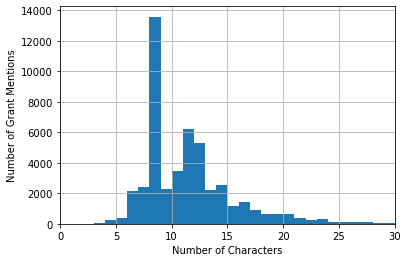
\includegraphics[scale=0.45]{grant_lens.png}
    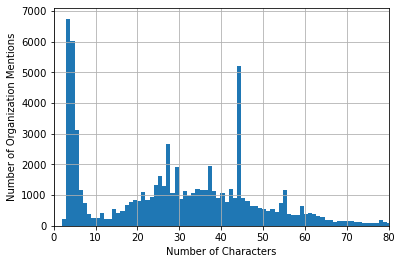
\includegraphics[scale=0.45]{org_lens.png}
    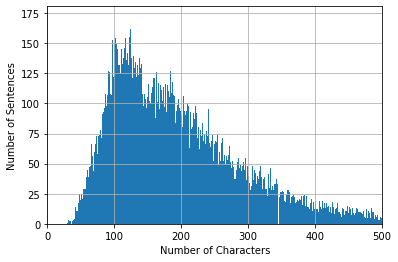
\includegraphics[scale=0.45]{sentence_lens.png}
    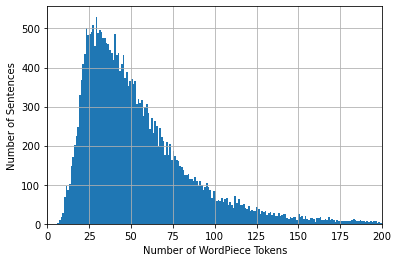
\includegraphics[scale=0.45]{sentence_tokens.png}
    \caption{Distribution of length of grant mentions (top-left), organization mentions (top-right), sentences (bottom-left) in terms of number of characters and distribution of number of tokens per sentence (bottom-right). Plots are cut over the x-axis, and the maximum x values are 75, 223, 9175 and 2760 respectively. Statistics obtained from Training and Validation$^1$ splits.}
    \label{fig:nerdatalen}
\end{figure}

\subsection{Evaluation}
\label{sec:NEReval}
To evaluate the Named Entity Recognition task, precision recall and F1 scores are used for each entity type, Organization and Grant. These metrics are defined in terms of True Positives (TP), False Positives (FP) and False Negatives (FN). Precision is defined as the fraction of TPs among all mentions extracted by the system, and recall is defined as the fraction TPs among all ground truth mentions. F1 score is the harmonic mean of precision and recall metrics. A mention is considered to be a TP if and only if both the extracted span and type information is correct. A FP corresponds to a mention that is extracted by the system wrongly, and a FN corresponds to a mention that is not extracted by the system while being present in the ground truth. This scheme is chosen as it is inline with evaluation of the CoNLL-2003 NER task \cite{conll}.
\subsection{Training}
\label{sec:trainingIthink}
In this section, the training and implementation details of the NER models are presented.
\subsubsection{Flair$^{NER}$}
The implementation of Flair$^{NER}$ is done using the Flair library \cite{flairlib}. In this library, both $LSTM^{forward}_{Flair}$ and $LSTM^{backward}_{Flair}$ trained on the 1 billion word corpus \cite{onebillion} are available. Using these and pretrained GloVe embeddings, the BiLSTM-CRF model is trained on the Training split and the progress is monitored on Validation$^1$ split using the training interface of Flair.  Mainly, the hyperparameters and training strategy reported in \cite{flairpaper} is followed, while changing minor things to address the computational limitations. The batch size was set to 8 and the model started training with a learning rate of 0.1. When for 2 epochs, no improvement on the Validation$^1$ split was observed, the learning rate was halved. The training is stopped when no improvement was made in a certain learning rate, amounting to 37 epochs in total. The performance on Validation$^1$ was measured as micro-averaged F1 score of the output tags. The models were saved at the end of each epoch, and the model that performed best on Validation$^1$ is selected

\subsubsection{BERT$^{NER}$ and BERT$^{NER}_{SC}$}

All parameters of BERT$^{NER}$ are fine-tuned end-to-end with different hyperparameter settings, using the Training split. The progress of training is monitored on Validation$^1$ across epochs, with respect to the same evaluation metric of the task (see Section \ref{sec:NEReval}).

Following BERT \cite{BERT}, BERT$^{NER}$ can also process a maximum of 512 tokens per input. Hence, the sentences having more tokens are split into smaller chunks, such that there is no overlap between chunks and no word is scattered across chunks. Later on, the predictions are merged as a postprocessing step. 

Devlin et al. (2019) \cite{BERT} suggested different hyperparameter settings for fine-tuning BERT: a batch size of 16 or 32, learning rate of $5\times10^{-5}$, $3\times10^{-5}$ or $2\times10^{-5}$; and training for 2, 3 or 4 epochs. Due to memory requirements, the batch size is set to 8. Then, the model is trained for 10 epochs with a learning rate of $2\times10^{-5}$, while saving the model at the end of each epoch. On top of that, 3 more models are trained using a linear learning rate scheduler for 2, 3 and 4 epochs respectively. The number of warmup steps is set to 50. For implementation, the library Transformers \cite{huggingface} by Hugging Face\footnote{\url{https://huggingface.co/}} is used. 

BERT$^{NER}_{SC}$ is trained with the exact same hyperparameter settings that produced the best results for BERT$^{NER}$. 

\section{Experiment 2: Entity Disambiguation for Funding Organizations}
\label{sec:EDExperiment}

\subsection{Preprocessing}
\textcolor{red}{say that the links to unknown entities are converted to NIL}
\textcolor{red}{explain NIL mentions}
\textcolor{red}{When we see Table \ref{tab:goldstatsed2} and \ref{tab:goldstatsed3}, it is possible to see that the entities we have in valid and test sets that are not in training set is longtail.}

\begin{table}[h!]
    \centering
    \begin{tabular}{ccccc}
    Dataset Split & \#Articles & \#ORG Mentions & \#Links & NIL Mentions  \\
    \hline
    Training & 29,118 & 95,761 & 77,972 & 18.58\% \\
    Validation$^1$ & 991 & 5,618 & 4,749 & 15.47\% \\
    Validation$^2$ & 3,943 & 19,765 & 16,689 & 15.56\% \\
    Test & 17,333 & 52,378 & 42,514 & 18.83\% \\ 
    \end{tabular}
    \caption{Dataset splits and statistics for ED. For each split, number of articles with at least one organization mention, number of organization mentions, number of mentions that are linked to an entity and the percentage of NIL mentions are shown.}
    \label{tab:goldstatsed}
\end{table}

\begin{table}[h!]
    \centering
    \begin{tabular}{cccc}
    Dataset Split & \# Unique Entities & Overlap with Training & KR Coverage\\
    \hline
    Training & 7,234 & - & 26.9\%\\
    Validation$^1$ & 1,222 & 88.63\% & 4.54\%\\
    Validation$^2$ & 2,658 & 81.6\% & 9.88\%\\
    Test & 5,590 & 71.91\%& 20.79\%\\
    \end{tabular}
    \caption{Dataset splits and number of unique entities in each split. Third column indicates the percentage of unique entities that are also present in the Training split for Validation$^1$, Validation$^2$ and Test splits. The last column shows the percentage of Knowledge Repository covered by each split.}
    \label{tab:goldstatsed2}
\end{table}

\begin{table}[h!]
    \centering
    \begin{tabular}{ccc}
    Dataset Split & \# Links & Links not in Training\\
    \hline
    Validation$^1$ & 4,749 & 3.39\% \\
    Validation$^2$ & 16,689 & 3.52\% \\
    Test & 42,514 & 5.14\% \\
    \end{tabular}
    \caption{Dataset splits and number of links. The third column shows the percentage of links for which the target entity do not exist as a link in the Training split.}
    \label{tab:goldstatsed3}
\end{table}



\begin{figure}[h!]
    \centering
    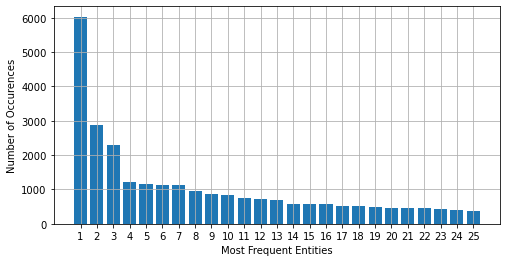
\includegraphics[scale=0.6]{ent_occ.png}
    \caption{Number of occurrences of top 25 most frequent entities. Statistics obtained using Training and Validation$^1$ splits.}
    \label{fig:entpopul}
\end{figure}

\subsection{Evaluation}
\subsection{Training}
\section{Experiment 3: Entity Linking for Funding Organizations}
\label{sec:ELExperiment} 
\subsection{Preprocessing}
\begin{table}[h!]
    \centering
    \begin{tabular}{ccccc}
     Dataset Split & \#Articles & \#ORG Mentions & \#Links & NIL Mentions  \\
     \hline
    Validation$^1$ & 1,000  & 4,622 & 3,954  & 14.45\% \\
    Validation$^2$ & 4,000  & 16,276 & 13,958 & 14.24\% \\
    Test           & 13,851 & 37,340 & 31,153 & 16.57\% \\
    \end{tabular}
    \caption{Dataset splits and statistics for EL. For each split, number of articles with at least one organization mention, number of organization mentions, number of mentions that are linked to an entity and the percentage of NIL mentions are shown.}
    \label{tab:goldstatsel}
\end{table}


\begin{table}[h!]
    \centering
    \begin{tabular}{cccc}
    Dataset Split & \# Unique Entities & Overlap with Training & KR Coverage\\
    \hline
    Validation$^1$ & 1,034 & 89.46\% & 3.85\%\\
    Validation$^2$ & 2,302 & 83.36\% & 8.57\%\\
    Test & 4,350 & 76\%& 16.18\%\\
    \end{tabular}
    \caption{Dataset splits and number of unique entities in each split. Third column indicates the percentage of unique entities that are also present in the Training split. The entities in the Training split is determined using the dataset for the ED task. The last column shows the percentage of Knowledge Repository covered by each split.}
    \label{tab:goldstatsel2}
\end{table}
26,892
\begin{table}[h!]
    \centering
    \begin{tabular}{ccc}
    Dataset Split & \# Links & Links not in Training\\
    \hline
    Validation$^1$ & 3,954   & 3.14\% \\
    Validation$^2$ &  13,958 & 3.19\% \\
    Test &            31,153 & 4.28\% \\
    \end{tabular}
    \caption{Dataset splits and number of links. The third column shows the percentage of links for which the target entity do not exist as a link in the Training split. The entities in the Training split is determined using the dataset for the ED task.}
    \label{tab:goldstatsel3}
\end{table}

\subsection{Evaluation}




\newpage
\chapter{Results}
\textcolor{red}{Get test set results for best models and baselines (Best NER, NER baseline; Best ED, ED baseline; Best NER+ED, EL Baseline. Rest is on Validation2 }

\section{Domain Adaptation of BERT}

To train BERT$_{SC}$, according to the initial setup, the Task-Adaptive Training was going to be performed for 2 epochs i.e. around 13,500 steps with a batch size of 2048 over 13,800,000 training samples. For this purpose, an NVIDIA Tesla K80 GPU with 12 GB of memory is used. However, it was observed that after 2 days of training, only 1000 steps were finished. Due to the time constraints, it was determined to stop the training at that point. After 1000 steps, a perplexity of 2.8612 is achieved on the Validation$^1$ set. Figure \ref{fig:perp} shows the change of perplexity on Validation$^1$, recorded every 20 training steps.

\begin{figure}[h!]
    \centering
    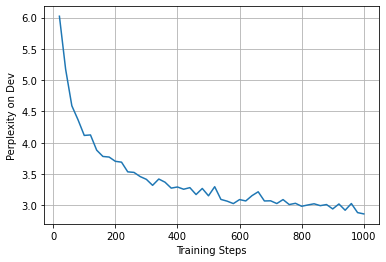
\includegraphics[scale=0.7]{perpplot.png}
    \caption{Perplexity on Validation$^1$ during training}
    \label{fig:perp}
\end{figure}

Based on the perplexity plot on Validation$^1$ and the results, we believe that it is possible to acquire a larger performance gain when the training with the full dataset is completed. However, this is left to future work due to time constraints and computational requirements. 

The next section compares NER models trained using BERT$_{BASE}$ and BERT$_{SC}$ to show the effectiveness of domain adaptation.

\section{Named Entity Recognition for Funding Bodies}
To compare the developed NER models, the current NER component of Elsevier, which is based on Stanford NER \cite{stanfordNER},  is used as a baseline.

For Flair$^{NER}$, a model selection was performed on the models that were saved at the end of each epoch using the $Validation^1$ dataset (see Section \ref{sec:trainingIthink}). At the end, the model at the end of 33 epochs is selected. The losses, scores and learning rates per epoch are presented in Appendix \ref{sec:app:flairner}. One epoch of training Flair$^{NER}$ took approximately 50 minutes on an NVIDIA Quadro T1000 GPU with 4GB memory. 

The training of BERT$^{NER}$ and BERT$^{NER}_{SC}$ is done using an NVIDIA Tesla K80 GPU with 12 GB of memory. On this device, one epoch took approximately 1 hour. After the experimentation with different hyperparameter settings, it was decided that training for 3 epochs with a linear learning rate scheduler produced the best results. Appendix \ref{sec:app:bertner} shows detailed results on this experimentation.

\begin{table}[h!]
    \centering
    \begin{tabular}{c| c c c| c c c}
    &\multicolumn{3}{c|}{Organization}&\multicolumn{3}{c}{Grant} \\
    System&Precision&Recall&F1&Precision&Recall&F1\\
    \hline
    Baseline & 73.699&	75.096&74.391&94.108&94.769&94.437
 \\[0.7ex]
    BERT$^{NER}$ & 79.183&86.029&82.464&94.711&97.389&96.031
\\[0.7ex]
    BERT$^{NER}_{SC}$ & 80.282&86.536&83.292&94.896	&97.627&96.242
  \\[0.7ex]
    Flair$^{NER}$& 85.827&78.018&81.736&97.557&95.24&96.385
 \\[0.7ex]
    \end{tabular}
    \caption{NER Results on Validation$^2$ split}
    \label{tab:all_ner_results}
\end{table}

Table \ref{tab:all_ner_results} compares the precision, recall and F1 scores for Organization and Grant mentions on Validation$^2$ dataset. It can be seen that all models perform well on extracting grant mentions, while Flair$^{NER}$ obtains the highest F1 score with a small difference. In contrast, using neural language model improve the performance on Organization mentions with a large margin, resulting in a minimum absolute increase of 7.4 points in terms of F1.

BERT$^{NER}$ sligtly outperforms Flair$^{NER}$ in terms of Organization F1-score by an increase of 0.7 points. However, the main difference is the precision and recall values. Flair$^{NER}$ achieves a precision that is 6.6 points higher than that of BERT$^{NER}$, while BERT$^{NER}$ achieves a recall that is 8 points higher. In funding data extraction, for NER component, a higher recall is preferred in this study due to two reasons. As the mention boundaries may be ambiguous, sometimes it may not be possible to match the Gold boundaries. And since the neural ED model utilizes the surrounding context of the mention, some missing tokens in the immediate context may not be very problematic. However, if a mention is missed completely, there is nothing that can be done about it.

BERT$^{NER}_{SC}$ improves upon BERT$^{NER}$ further, showing the importance of domain adaptation. When trained with the exact same setup, it is possible to see an improvement of 1 points in precision and 0.5 points in recall. At the end, it is decided to use BERT$^{NER}_{SC}$ as the NER component to extract mentions of funding bodies. Table \ref{tab:all_ner_results_test} compares the results of BERT$^{NER}_{SC}$ and Elsevier Baseline on the Test split. It is possible to see that the performance gain persists on the Test split as well. \textcolor{red}{Hence, it is concluded that this work improved upon Elsevier's NER baseline by X points gain in precision and Y points gain in recall.}

\begin{table}[h!]
    \centering
    \begin{tabular}{c| c c c| c c c}
    &\multicolumn{3}{c|}{Organization}&\multicolumn{3}{c}{Grant} \\
    System&Precision&Recall&F1&Precision&Recall&F1\\
    \hline
    Baseline &  76.166 & 72.871  & 74.482 & 93.371   & 93.238  & 93.305
 \\[0.7ex]
    BERT$^{NER}_{SC}$ & 
  \\[0.7ex]
    \end{tabular}
    \caption{NER Results on Test split}
    \label{tab:all_ner_results_test}
\end{table}

\section{Entity Disambiguation for Funding Organizations}

\begin{table}[h!]
    \centering
    \begin{tabular}{c|ccc|ccc}
    &\multicolumn{3}{c|}{Micro-Averaged}&\multicolumn{3}{c}{Macro-Averaged}\\
    System  & Precision & Recall & F1 & Precision & Recall & F1   \\
    \hline
    Els. Baseline     & &&&&&\\
    Commonness   &&&&&&\\
    BiEncoder  &&&&&&\\
    \end{tabular}
    \caption{Caption}
    \label{tab:my_label}
\end{table}

\section{Entity Linking for Funding Organizations}


\begin{table}[h!]
    \centering
    \begin{tabular}{cc|ccc|ccc}
    &&\multicolumn{3}{c|}{Micro-Averaged}&\multicolumn{3}{c}{Macro-Averaged}\\
    NER & ED  & Precision & Recall & F1 & Precision & Recall & F1   \\
    \hline
    Els. Baseline & Els. Baseline     & &&&&&\\[0.7ex]
    Els. Baseline & Commonness        &&&&&&\\[0.7ex]
    Els. Baseline & BiEncoder         &&&&&&\\[0.7ex]
    BERT$_{SC}^{NER}$ & Els. Baseline     & &&&&&\\[0.7ex]
    BERT$_{SC}^{NER}$ & Commonness        &&&&&&\\[0.7ex]
    BERT$_{SC}^{NER}$ & BiEncoder         &&&&&&\\[0.7ex]
    \end{tabular}
    \caption{Caption}
    \label{tab:my_label}
\end{table}

\begin{table}[h!]
    \centering
    \begin{tabular}{c| c c c c c c}
    &\multicolumn{3}{c}{Organization}&\multicolumn{3}{c}{Grant} \\
    System&Precision&Recall&F1&Precision&Recall&F1\\
    \hline
    Els. Baseline & &&&&& \\[0.7ex]
    BERT$^{NER}_{SC}$ & &&&	&& \\[0.7ex]
    \end{tabular}
    \caption{Test results for Named Entity Recognition}
    \label{tab:trner}
    
    
    
    \vspace*{0.5cm}\begin{tabular}{c|ccc|ccc}
    &\multicolumn{3}{c|}{Micro-Averaged}&\multicolumn{3}{c}{Macro-Averaged}\\
     System  & Precision & Recall & F1 & Precision & Recall & F1   \\
    \hline
    Els. Baseline      & &&&&&\\[0.7ex]
     ?         &&&&&&\\[0.7ex]
    \end{tabular}
    \caption{Test results for Entity Disambiguation}
    \label{tab:tred}
    
    \vspace*{0.5cm}\begin{tabular}{c|ccc|ccc}
    &\multicolumn{3}{c|}{Micro-Averaged}&\multicolumn{3}{c}{Macro-Averaged}\\
     System  & Precision & Recall & F1 & Precision & Recall & F1   \\
    \hline
    Els. Baseline      & &&&&&\\[0.7ex]
    ?         &&&&&&\\[0.7ex]
    \end{tabular}
    \caption{Test results for Entity Linking}
    \label{tab:trel}
    
\end{table}





\chapter{Discussion}
Put Limitations here.

I can also put some error analysis here
\section{Comparison of BERT$^_{NER}$ and Flair$^_{NER}$}
\begin{itemize}
    \item  Talk a bit about precision/recall tradeoff of the results
    \item Error analysis eg. "for" as org, maybe CRF may help.
    \item Tell why recall is more important (the mention boundaries are sometimes ambigious and the linker utilizes the context anyway. Maybe give an example for the former, sth like "NSF" vs "NSF of USA"
    \item ert may be unnecessary for grant numbers, but it is nice to see that it is working with them so we do not need two separate models for org and grant mentions
    \item Training time much longer with Flair. This wouldnt change even though a more powerful GPU is used (show that even if the other GPU fastened the process x3 times, it is still a lot slower)
\end{itemize}

\section{BERT$_{SC}$}
\begin{itemize}
    \item Compare perplexity numbers these with BERT paper and dontstop paper
    \item Say that performance may further be improved if more data is used to pretrain BERTSC (based on the perplexity plot)
\end{itemize}


\chapter{Conclusion}
Put Future Work somewhere.



\newpage
\bibliographystyle{plain}
\bibliography{references.bib}



\appendix
\newpage
\chapter{NER Data Preprocessing}
\label{app:NERPrepro}
 Below, you may find the steps to assign labels to tokens using the gold annotations in sequential order.
\begin{enumerate}
    \item Label tokens of ORG mentions. Sometimes, annotators tend to extract mentions not as a continuous span, but rather a list of individual words. If there more than two characters in-between, take the first continuous set of words. The decision of not taking the mention from the first annotated word until the last is based on the cases where there are too many characters or grant mentions in-between these words. It was observed that the first span mostly contained the important words to be able to identify the organization. Example annotations where underlined text corresponds to a single mention based on the gold annotation:
    \begin{quote}
        (a) \underline{National Instituteo f Child Healtha ndH umanD evelopmen} \underline{t} \\
        (b) the \underline{Technological Innovation and Demonstration of Social Undertakings} \underline{Project fund} ( HS2014003 ) of \underline{Nantong, Jiangsu}, China;
    \end{quote}

    \item Remove duplicate ORG mentions based on their position on text. If there are two mentions with same text in different parts of the input, both are kept.
    \item Remove ORG mentions that are too long. Very rarely, the annotators extracted too large of a span as a mention, sometimes even the whole article. ORG mentions longer than $200$ characters are discarded.
    \item If there are overlapping ORG mentions, keep only the one with the largest span. Example overlapping gold annotations:
    \begin{quote}
        (a) ``National grant no. Science NSC Council'' \\
        (b) ``NSC''
    \end{quote}
    \item Label tokens of GRT mentions. Follow the same rule as the first step for mentions that are not continuous spans.
    \item Remove duplicate GRT mentions similar to the second step.
    \item Discard the grant mentions that are longer than $100$ characters. 
    \item Resolve overlapping GRT mentions similar to the fourth step.
    \item Resolve overlapping ORG and GRT mentions. Keep the label of the ORG mention, if there are tokens left on the right-hand-size, label them as GRT. 
    \begin{quote}
        Text: ``supported by the European Community, FP6 036097-2'' \\
        (a) ORG Mention: ``European Community, FP6'' \\
        (b) GRT Mention: ``FP6 036097-2'' \\
        (c) Span that is labelled as ORG: ``European Community, FP6'' \\
        (d) Span that is labelled as GRT: ``036097-2''
    \end{quote}
\end{enumerate}
    As the candidate models for NER were BERT-based \cite{BERT} and Flair-based \cite{flairpaper} models, the tokenizers these models use were tried for the tokenization of the input text before assigning the NER labels. After empirical analysis, it was decided the use the tokenizer of the case-sensitive BERT$_{BASE}$ model \cite{BERT}, as it was splitting the text to smaller pieces, which was crucial to minimize labelling errors. One drawback of this tokenizer is that it being a word-piece tokenizer. Hence, it also splits some words into smaller pieces based on the vocabulary of the model. As a post-processing step, these wordpieces are merged back together. The choice of using the same tokenizer through all NER models is to eliminate any effect that can be caused by using different tokenizers during comparison.

\newpage
\chapter{Training Details}
\section{BERT$_{SC}$}
\label{sec:app:bertsc}
The table below shows the hyperparameters for Task-Adaptive Pretraining.
\begin{table}[h!]
    \centering
    \begin{tabular}{|lc|}
    \hline
     Number of Epochs: & 2  \\
     Batch Size: & 4\\
     Effective Batch Size: & 2048 \\
     Maximum Learning Rate: & 0.0005 \\
     MLM Probability & 0.15 \\
     Max. Gradient Norm & 1 \\
     Optimizer & Adam \cite{adamopt} \\
     Learning Rate Scheduler & Linear \\
     Warmup Steps & 0 \\
     Weight Decay & 0 \\
     Adam Epsilon & 10$^{-8}$ \\
     Seeds & 0 \\

     \hline
    \end{tabular}
    \caption{Hyperparameters for Task-Adaptive Pretraining}
    \label{tab:pretrainhyper}
\end{table}
\newpage
\section{Flair$^{NER}$}
\label{sec:app:flairner}
Figure \ref{fig:flairtrain} shows the $Training$ and $Validation^1$ losses, learning rate and $Validation^1$ scores over epochs. 
\begin{figure}[H]
    \centering
    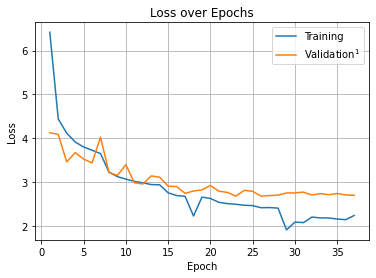
\includegraphics[scale=0.45]{flair_loss.png}
    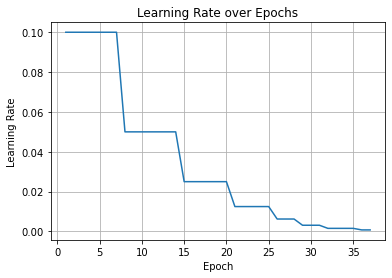
\includegraphics[scale=0.45]{flair_lrs.png}
    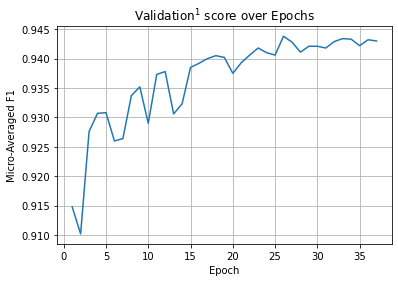
\includegraphics[scale=0.45]{flair_scores.png}
    \caption{Losess (up-left), learning rate (up-right) and $Validation^1$ scores (bottom) per epoch}
    \label{fig:flairtrain}
\end{figure}
\newpage
\section{BERT$^{NER}$}
\label{sec:app:bertner}
The tables below show the results of the models for each hyperparameter configuration on Validation$^2$ dataset. Table \ref{tab:bert_ner_no_scheduler} displays the results where the model was trained for 10 epochs and saved at the end of each. The Validation$^2$ results are obtained on specific epochs: 2, 3, 4, 6 and 10. 2, 3 and 4 are included as they were among the recommended hyperparameters. Epoch 6 and 10 are included as the former resulted in the highest Validation$^1$ ORG-F1 score while the latter was the last epoch. Table \ref{tab:bert_ner_scheduler} shows the results on Validation$^2$ dataset for the setting where a linear learning rate scheduler is used.

\begin{table}[h!]
    \centering
    \begin{tabular}{c| c c c| c c c}
    &\multicolumn{3}{c|}{Organization}&\multicolumn{3}{c}{Grant} \\
    Epoch&Precision&Recall&F1&Precision&Recall&F1\\
    \hline
    2     & 80.38	&84.139&82.217	&94.179&	96.954&95.546  \\
    3     & 78.759	&84.904&81.716	&94.514&	96.776&95.632  \\
    4     & 79.175	&84.176&81.599	&94.302&	96.885&95.576  \\
    6     & 79.879	&84.714&82.226	&94.73	&96.529&95.621  \\
    10   &  81.036	&80.238&80.635	&94.621&	96.381&95.493  \\
    \end{tabular}
    \caption{BERT$^{NER}$ results on Validation$^2$. Trained for 10 epochs without a scheduler, the model is saved after every epoch.}
    \label{tab:bert_ner_no_scheduler}
\end{table}


\begin{table}[h!]
    \centering
    \begin{tabular}{c| c c c| c c c}
    &\multicolumn{3}{c|}{Organization}&\multicolumn{3}{c}{Grant} \\
    Epoch&Precision&Recall&F1&Precision&Recall&F1\\
    \hline
    2     & 78.444&	85.796&	81.955&	94.594&	97.429&	95.991
 \\
    3     & 79.183&86.029&82.464&94.711&97.389&96.031
 \\
    4     & 79.409&85.876&82.516&94.947&97.379&96.148
 \\
    \end{tabular}
    \caption{BERT$^{NER}$ results on Validation$^2$. Trained for 2,3 and 4 epochs respectively with a scheduler, the model is saved after the training is done.}
    \label{tab:bert_ner_scheduler}
\end{table}

As the scores for Grant mentions are high in each setup, the model is chosen based on the scores on Organization mentions. Recall is favored over precision since the mention boundaries can sometimes be subjective, and the ED utilizes the surrounding context anyway. Based on this intuition, the model that is trained for 3 epochs with a learning rate scheduler is selected. This model has the highest recall for Organization mentions and the second highest F1 score. Hence, BERT$^{NER}_{SC}$ is also trained with this hyperparameter setup.

\end{document}

